\documentclass{article}

%paquetes necesarios
\usepackage{graphicx} %para incluir gráficos
\usepackage{amsmath} %para fórmulas matemáticas
\usepackage{booktabs} %para tablas
\usepackage{blindtext}
\usepackage{hyperref}
\usepackage[spanish]{babel}
\usepackage{graphicx}
\usepackage{subcaption}
%título del informe
\title{Informe sobre el dataset Data Science Salaries 2023}
\author{Borgo Martin, Sandoval Jose, Molina Leandro}
\hypersetup{
	colorlinks=true,
	linkcolor=blue,
	filecolor=magenta,      
	urlcolor=cyan,
	pdftitle={Overleaf Example},
	pdfpagemode=FullScreen,
}

\begin{document}
	
	%creación del título
	\maketitle
	\begin{abstract}
		El informe analiza el conjunto de datos de salarios de ciencia de datos del año 2023 de Kaggle, proporcionando un análisis detallado de las variables incluidas en el conjunto de datos y comparación con otro conjunto de datos. Se utilizó Python y Excel para la realización de gráficos y tablas. Este informe proporciona información para los profesionales de la ciencia de datos y los interesados en comprender el mercado actual.
	\end{abstract}
	\pagebreak
	\vspace{-20pt}
	
	\noindent
	\tableofcontents
	\pagebreak
	%introducción
	\section{Introducción}
	Los trabajos para la ciencia de datos (data science) continúan en crecimiento, y las organizaciones están compitiendo para contratar a los expertos de la materia. Con el objetivo de entender este ambiente, se ha creado el siguiente informe. Este informe tiene como objetivo proporcionar un análisis a los datos obtenidos, que incluye información sobre la experiencia, el tipo de empleo, el cargo y la ubicación geográfica de los profesionales de la ciencia de datos, así como la moneda en la que se les paga, como también un análisis a la distribución de los salarios (usando coeficiente de Gini) y se termina comparando con otro dataset del mismo ámbito. Se espera ayudar a los profesionales o interesados del mercado data science a que comprendan las tendencias del mercado laboral.
	%resultados
	\section{Dataset Utilizado}
	Para este informe se utiliza el dataset proporcionado por kaggle\footnote{\href{https://www.kaggle.com/datasets/arnabchaki/data-science-salaries-2023}{Véase: Salaries of Different Data Science Fields in the Data Science Domain}}Es una plataforma que aloja competencias de aprendizaje automático, conjuntos de datos públicos y privados, y herramientas de exploración y análisis de datos. Este dataset contiene información sobre los salarios de data science y en diversos países del mundo. El conjunto de datos incluye varias variables, como el año de trabajo, el nivel de experiencia, el tipo de empleo, el título del trabajo, el salario bruto total pagado, la moneda en la que se pagó el salario y el salario en USD. También incluye información sobre el país de residencia del empleado, la cantidad de trabajo realizado de forma remota, la ubicación del país de la empresa y el tamaño de la empresa. Es un dataset confiable ya que ningún dato es “nulo”.\footnote{ \href{https://www.kaggle.com/code/mudassarshaheen/data-science-salaries-eda-visualization}{Véase: en la sección basic exploring.}}
	
	\section{Análisis de variables y realización de gráficas}
	A continuación se analizaran la distribución de los salarios en dólares de acuerdo a la experiencia laboral\footnote{En el dataset están referidos como:
		\\EN, que se refiere a Entry-level / Junior
		\\MI, que se refiere a Nivel medio / Pre-Senior.
		\\SE, que corresponde a Senior-level / Experto.
		\\EX, que se refiere a nivel ejecutivo / Director.} de cada uno de los encuestados (que participaron del dataset) que pertenecen al sector del Data Science, cada nivel de experiencia será evaluado mediante una gráfica de cajas resulta muy útil a la hora de determinar los sesgos y la dispersión de los datos, además de ofrecer información sobre la media y la mediana. Se calcularon las medias aritméticas y medianas para cada nivel de experiencia por el salario en dólares véase la \hyperref[tabla 1.1]{Tabla 1.1}.
	En la \hyperref[figura 1.1 diagrama]{figura 1} se representa la distribución de los salarios de los analistas Junior (320) que forman parte de la muestra. A simple vista podemos notar que la distribución de los datos posee un gran sesgo positivo, eso quiere decir que los datos están más agrupados por debajo de la media.
	Realizando un análisis más riguroso con esos datos encontraremos que la mediana es 70000, esto significa que el 50\% (106) de los trabajadores Juniors se encuentran cobrando menos de ese monto y el 50\% restante más de ese monto. En este caso, como en los que veremos a continuación, la mediana resulta mucho más representativa, ya que la media se ve afectada por los valores altos como 300000 o 220000. Por lo tanto, la media no puede considerarse una buena medida para representar este conjunto de datos.
	Enfocándonos esta vez en la dispersión de los datos, si calculamos la desviación estándar, nos arrojará 52225.42 como resultado. Antes de seguir el desarrollo conviene hacer una aclaración sobre esto, debido a que estamos analizando salarios anuales en dólares y considerando los datos que se muestran en la \hyperref[figura 2 torta]{figura 2}, donde vemos que el 95\% de los encuestados actualmente residen en países donde las rentas son elevadas, consideramos que una desviación estándar de 10000 es buena en este caso.
	Con este punto aclarado podemos afirmar entonces que: 
	\begin{enumerate}
		\item Los datos de la \hyperref[figura 1.1 diagrama]{figura 1.1} están muy dispersos en esa distribución.
		\item Debido a lo antes mencionado la media tampoco es muy representativa para ese conjunto de datos.
	\end{enumerate}
Pasa algo muy similar en las figuras \hyperref[figura 2.2 diagrama]{2.2} y \hyperref[figura 3.1 diagrama]{la 3.1}, donde se representan a los empleados con un nivel Pre-Senior (805) y Senior (2516) respectivamente. Si bien presentan algunas cualidades diferentes como el hecho de que en ambas figuras existe un sesgo positivo pero es casi mínimo en comparación con la primera gráfica analizada. Sucede lo mismo, la desviación estándar es extremadamente alta 54387.68 y 52225.42 respectivamente, lo que al igual que la distribución anterior deja a la media aritmética casi sin mucha importancia, sin contar que las gráficas que estamos observando ahora cuentan con mucho más valores atípicos, un segundo motivo para descartar a la media. Este mismo hecho se repite para la \hyperref[figura 4.1 diagrama]{figura 4}, donde están representados los analistas expertos, con la particularidad de que, al contrario que las distribuciones presentadas anteriormente, las cuales poseen un sesgo positivo; esta aparenta ser simétrica, porque si nos ponemos estrictos la media y la medina tendrían que ser las mismas para ser considerada simétrica, cosa que no pasa aquí tampoco. Hay que tener en cuenta que de todas las muestras analizadas esta última es la que menor cantidad de datos tiene (114), en comparación con las demás que tienen muestras mucho mayores. Es probable que a medida que vayamos agregando más datos a este grupo la distribución de estos mismos irá cambiando.
Algo a destacar es la dominancia de Estados Unidos en cantidad de empleados residiendo en su país, en la \hyperref[figura 5.1 grafico de barras agrupado]{figura 5.1} donde se agrupan la cantidad de encuestados agrupados según los 5 países donde hay más residencia, discriminados a su vez según experiencia laboral, y \hyperref[tabla 1.3]{tabla 1.3} donde se muestra los datos brutos con los que se construyó la gráfica. En esa tabla podemos ver la dominancia estadounidense en los 4 niveles de experiencia comparado con los 4 países con mayor cantidad de residentes (como también el total de empleados).
	\section{Desigualdad e igualdad en salarios en ciencia de datos.}
	\section{Figuras y tablas.}
	
	\begin{figure}[htbp]
		\centering
		\begin{subfigure}[b]{1.1\textwidth}
			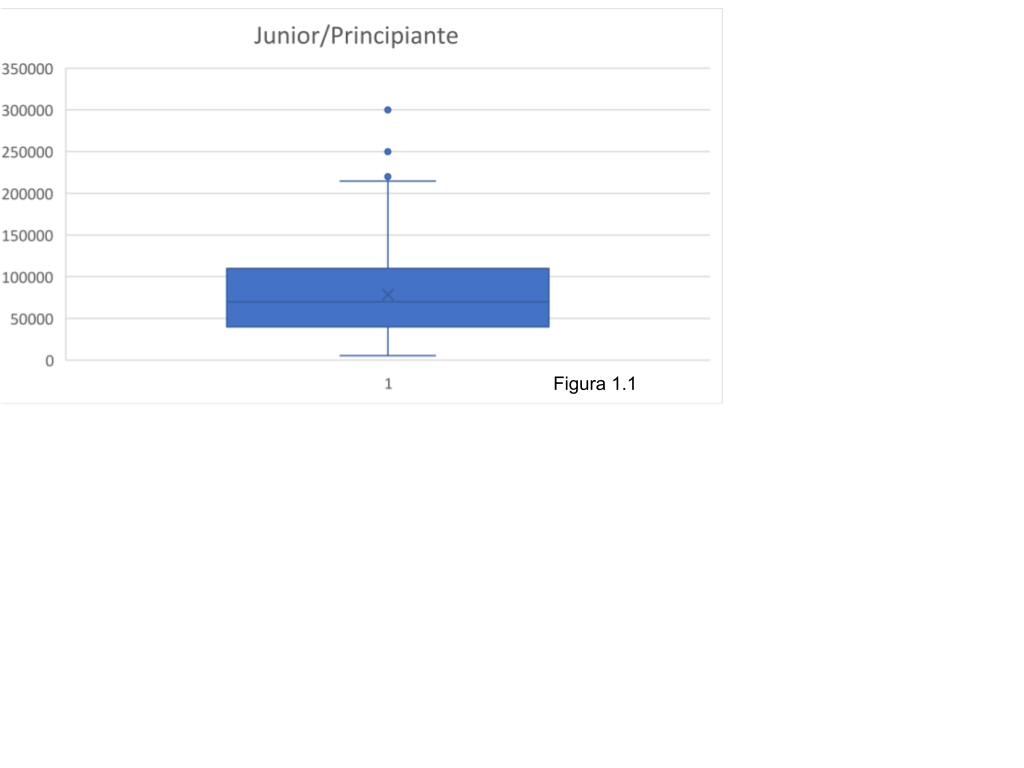
\includegraphics[width=\textwidth]{FigurasTablas/figura1.1diagrama}
			\label{figura 1.1 diagrama}
		\end{subfigure}

		\begin{subfigure}[b]{1.1\textwidth}
			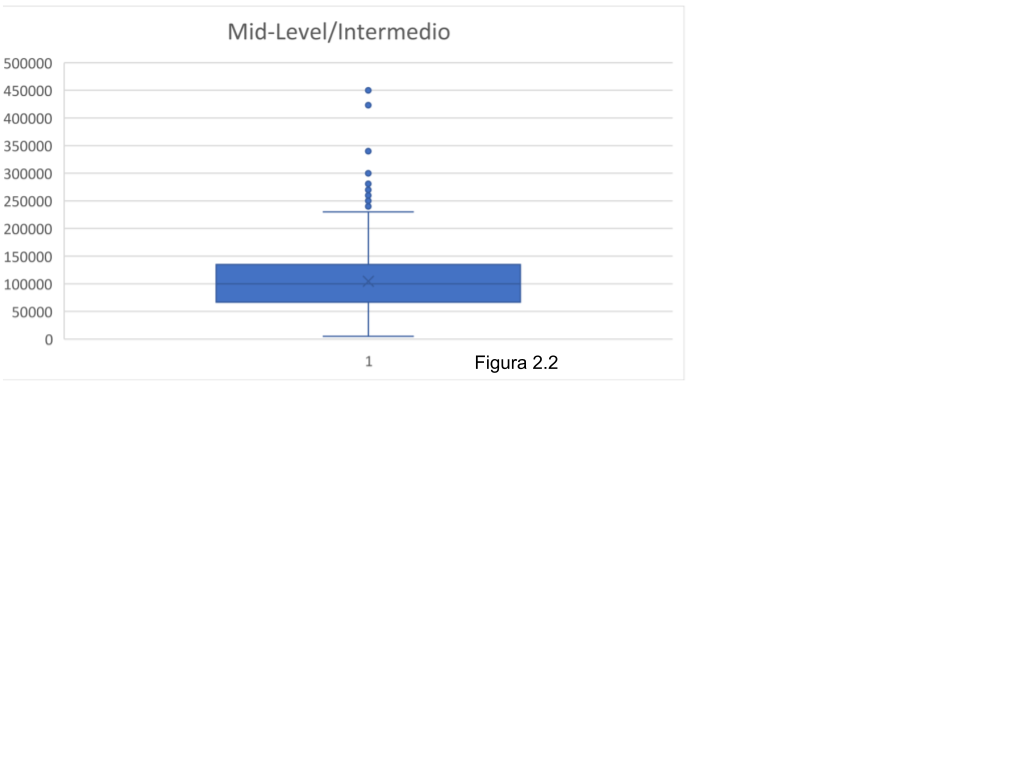
\includegraphics[width=\textwidth]{FigurasTablas/figura2.2diagrama.png}
			\label{figura 2.2 diagrama}
		\end{subfigure}
		
	\end{figure}

	\begin{figure}
		\begin{subfigure}[b]{1.1\textwidth}
			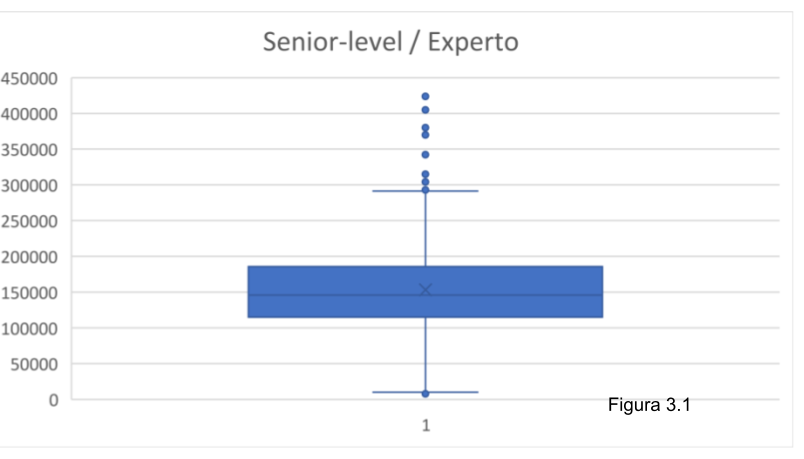
\includegraphics[width=\textwidth]{FigurasTablas/figura3.1diagrama.png}
			\label{figura 3.1 diagrama}
		\end{subfigure}	
		
		\begin{subfigure}[b]{1.1\textwidth}
			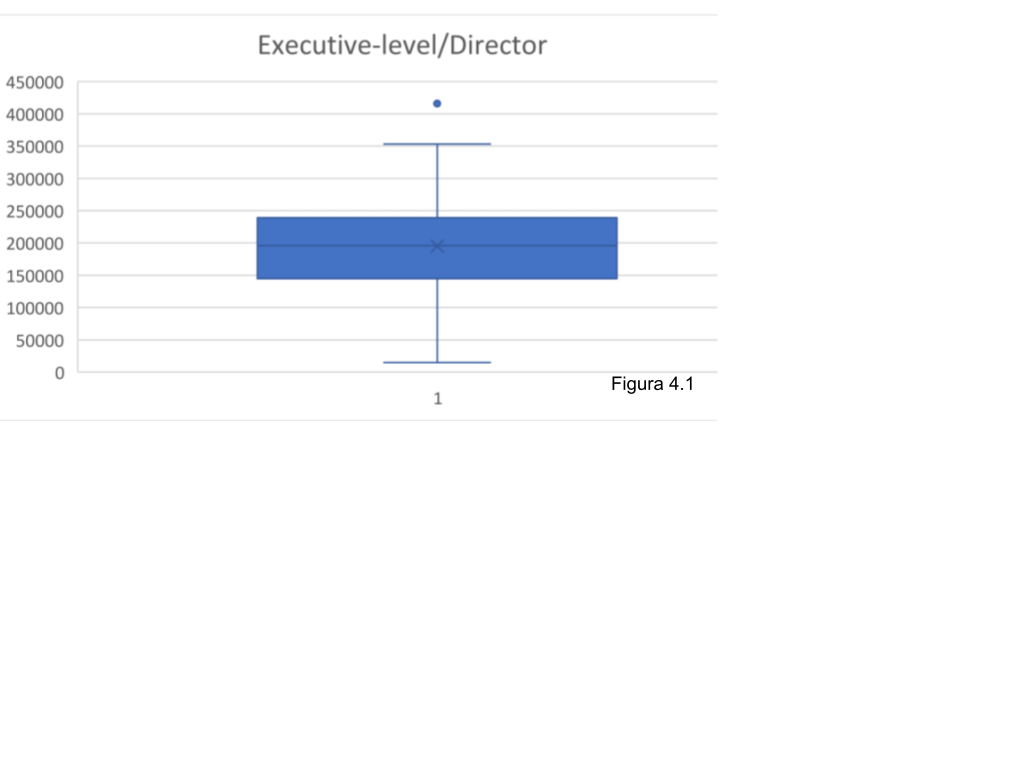
\includegraphics[width=\textwidth]{FigurasTablas/figura4.1diagrama.png}
		\end{subfigure}	
	\end{figure}

	%\label{figura 1.1 diagrama}
	%\label{figura 2.1 torta}
	%\label{figura 2.2 diagrama}
	%\label{figura 3.1 diagrama}
	%\label{figura 4.1 diagrama}
	%\label{figura 5.1 grafico de barras agrupado}
	%\label{tabla 1.1}
	%\label{tabla 1.2}
	%\label{tabla 1.3}
\end{document}
